\documentclass[11pt,letter]{article}
\usepackage[top=1.00in, bottom=1.0in, left=1.1in, right=1.1in]{geometry}
\renewcommand{\baselinestretch}{1.1}
\usepackage{graphicx}
\usepackage{natbib}
\usepackage{gensymb}
\usepackage{amsmath}
\usepackage{lineno}
\usepackage{xr-hyper}
\externaldocument{limitingcues_supp}

\def\labelitemi{--}
\parindent=0pt

\usepackage{Sweave}
\begin{document}
\bibliographystyle{/Users/Lizzie/Documents/EndnoteRelated/Bibtex/styles/besjournals} % change to pnas to count refs
\renewcommand{\refname}{\CHead{}}
\begin{flushright}
Version dated: \today
\end{flushright}
\bigskip
\noindent RH: Interactive cues \& phenology
% put in your own RH (running head)

\bigskip
\medskip
\begin{center}

% Insert your title:
\noindent{\Large {\bf How interactive effects of temperature and photoperiod shape spring plant phenology responses to warming}}\\ % OR How interactive cues will shape non-linear climate change responses ? 
% Concept paper on understanding interactive cues and climate change (with growth chamber studies) 
\bigskip

\noindent {\normalsize \sc
E. M. Wolkovich$^{1,2}$, C. J. Chamberlain$^{1,2}$, D. M. Buonaiuto$^{1,2}$, A. K. Ettinger$^{3}$ \\ \& I. Morales-Castilla$^{5}$}\\ % The lab in 2017 -- Lizzie, Ailene, Cat, Dan, Nacho

\noindent {\small \it
$^1$ Forest \& Conservation Sciences, Faculty of Forestry, University of British Columbia, 2424 Main Mall, Vancouver, BC V6T 1Z4\\
$^2$ Arnold Arboretum of Harvard University, 1300 Centre Street, Boston, Massachusetts, 02131, USA\\
$^3$ Organismic \& Evolutionary Biology, Harvard University, 26 Oxford Street, Cambridge, Massachusetts, 02138, USA\\
$^4$ The Nature Conservancy, 74 Wall Street, Seattle, Washington USA\\
$^5$ Global Change Ecology and Evolution Group, Department of Life Sciences, University of Alcal\`a, Alcal\`a de Henares 28805, Spain}
\end{center}
\medskip
\noindent{\bf Corresponding author:} Lizzie, see $^{3}$ above ; E-mail: e.wolkovich@ubc.ca\\


% 181 words; 94 refs on 2 April 2021
\begin{abstract} Climate change has advanced plant phenology globally 4-6 days per $\degree$C on average, with some species shifting much more. Such shifts have been some of the most reported and predictable biological impacts of rising temperatures. Yet as climate change has marched on, phenological shifts have appeared muted over recent decades---failing to match simple predictions of an advancing spring with continued warming. The main hypothesis for these changing trends is that other cues of spring phenology---long-documented in lab environments---are playing a greater role in natural environments due to climate change. Here we argue that accurately linking shifts observed in long-term data to underlying phenological cues requires greater integration of controlled environment experiments  with long-term data and insights from physiology. We highlight how seven decades of research in controlled environments can improve predictions for when, where, and how the interactive effects of other cues will impact simple linear predictions. At the same time a new generation of lab experiments could transform our fundamental understanding of phenology and improve forecasts of shifting phenology across different regions for decades to come. % Change tone here to -- we need better understanding of these other cues if we want to understand shifts across space and time. 
\end{abstract}

% \noindent \emph{Main message (and, really, it's important):} If you want to project climate change impacts, you need to focus on relevant changes in all three cues. The relevant changes part is about comparing cues, the all three cues is about interactive cues.
% Old abstract (2019 one):
% ... most predictable biological impacts of climate change. This predictability comes from decades of research, which have outlined the major cues that drive most studied plant phenology: temperatures (including spring warming and winter chilling) and daylength. Further simplifying predictions, spring temperatures are often the dominant cue in nature, making linear models of heat sums often excellent at predicting interannual variation in phenology. Yet as climate change has marched on, new research has uncovered possible failures to predict the current observed changes; increasingly, phenological shifts appear more muted over recent decades, or in certain locations. Here we argue that some of these inaccurate predictions are due to simple models that neglect to consider other major cues---especially winter chilling and daylength, which moderate and shape plant phenological responses to spring warming. We highlight how over 70 years of research in controlled environments can improve predictions for when, where and how the interactive effects of other cues will impact simple linear predictions. Finally, we discuss how a new generation of controlled environment experiments could rapidly improve our predictive capacity for woody plant phenology in coming decades.  

\noindent \emph{Keywords:} phenology, climate change, spring warming, chilling, forcing, daylength, photoperiod, non-linear responses, leafout, budburst\\

\newpage
\linenumbers
\section{Main text} % Currently about 4422 words with embedded refs; estimated words when using numbered refs (about 375 words in in-text citations)
Shifts in spring plant phenology are one of the most reported and predictable changes with climate change. Decades of research have documented advancing budburst, leafout and flowering with climate change \citep{delpierre2009, yu2010,Ellwood2012,jochner2013,hereford2017}, especially in temperate systems where long-term records highlight how humans have altered the timing of spring \citep{Schwartz:1997nn,Menzel2003a,menzel2006}. Recently, however, these advances have appeared to slow \citep{fu2015} or even reverse \citep{yu2010}---failing to match simple predictions of an advancing spring with continued warming \citep{Ellwood2012}. The main hypothesis for this failure is that spring warming---which most observational studies focus on---is no longer the only environmental cue that matters to predicting responses to warming \citep{chuine2016,gauzere2019}.\\

Despite the strong focus of spring phenology research on spring temperatures, increasing evidence suggests a more complicated underlying physiology for most plant species \citep[e.g.,][]{zohner2016,gauzere2019,ettinger2020}. For many species three major cues underlie spring phenology: forcing (warm temperatures, generally occurring in the late winter and early spring), chilling (cool temperatures, generally occurring in the fall and winter), and photoperiod (daylength). \\

Together, forcing, chilling and photoperiod may produce non-linear responses that many current methods do not predict, but observational studies have reported recently \citep{fu2015}. Predicting these non-linearities is a common goal in plant phenology research today \citep{gusewell2017,martlusch2017,gauzere2019,chen2019,keenan2019}, but has been slowed by data gaps and the underlying complexity of spring phenology. \\

The first step towards improved phenological predictions is robust measurements of chilling, forcing and photoperiod cues. Recently, efforts have focused on estimating these cues from long-term observational data \citep{Luedeling2009,lued2013diff}. Yet observational studies may struggle to robustly estimate any of the three major cues due to two types of statistical issues. First, in most observational data these cues correlated: forcing increases alongside longer photoperiods \citep{sarahailene2020}, and changes to chilling and photoperiod cues with warming predict the same response---later spring phenology. Approaches that attempt to disentangle some of these correlations, such as leveraging trends across elevation or latitude, may run afoul of other correlations \citep[][]{tansey2017}. Second, most observational studies focus on linear models of each cue, often without interactions between cues \citep{visser2001,polgar2014,asse2018}.\\ % Approaches that attempt to disentangle some of these correlations, such as leveraging trends across elevation or latitude, may run afoul of other correlations; for example, gradients in local adaptation can create shifts in the underlying cues along environmental gradients in complex ways

% Ailene writes ... I'm not sure if this is the best place for this paragraph. After reading the previous paragraph and this one I was left wondering- are we saying that linear models are problematic or that they are ok? Or are we saying they might be problematic but they might be ok- we don't know? It might be worth begin explicit about this. something like: "one the one hand, interactions between cues can affect phenology (e.g.), so excluding these interactions between cues may be problematic. On the other hand, using simple linear models with observational data..."
% Using simple linear models with observational data may make sense as phenological responses to most cues are expected to be linear except at the extremes. Natural conditions often see only a small slice of the range of values of each cue that are possible---and those values often appear to be in the middle---potentially linear---range \citep{gauzere2017,ettinger2020}. Further, given that interactions between cues are difficult to estimate---more so when those cues are highly correlated in nature---focusing on the main effects of cues may provide more robust estimates from observational data  \citep[main effects integrate over any interactions and require lower statistical power to robustly estimate compared to interactions,][]{gelman2006}. \\

In contrast to the limitations of observational studies, one method is designed to measure the complexity of cues: controlled environment (e.g., growth chamber) studies. Such studies have been conducted for over 70 years and are designed to understand nonlinear responses to warming. In contrast to observational studies, controlled environment studies can manipulate all three cues, extend to other cues that may be important in some species or biomes (e.g., humidity, drought conditions, light spectra), and can tease out interactions between cues by experimentally decoupling them.\\

Despite the prevalence of controlled environment studies on spring phenological cues, they have rarely been reviewed. Perhaps more surprisingly, they are often poorly integrated into the current phenological literature on climate change, including in debates where they are critical \citep[e.g.,][]{fu2015,richardson2018}.\\ % Could add back: "This includes in debates where they are critical, such as the importance of photoperiod in altering how warming affects phenology."

Here, we show how harnessing decades of controlled environment studies could transform our fundamental understanding of phenology and advance forecasting. We begin by outlining how the three major phenological cues---forcing, chilling and photoperiod---can produce non-linearities and how they will shift in coming decades with anthropogenic climate change. We then synthesize controlled environment studies to quantify how much of the cue-space (i.e., the possible range of each cue and interactions across cues) has been studied and how treatments compare to shifts in cues caused by climate change. Based on this, we outline a cross-disciplinary path forward where advances in physiology, greater integration of controlled environment studies with forecasting, and multi-species modeling can yield more robust predictions.\\

Given our aim to improve understanding of current trends and forecasts we focus on early vegetative phases (budburst and leafout), which are critical to plant growth and carbon storage, have been studied the most in experiments (see Supporting Information), and have shifted most with climate change \citep{Cleland:2007or,IPCC:2014sm}. We touch on other areas of research, which have been important to our understanding of the cues underlying phenology. In particular, research has been especially strong in model systems (e.g., \emph{Arabidopsis, Populus}) and crops \citep{cesaraccio2004}---with the exact phenophase of interest varying (more focus on germination and flowering in \emph{Arabidopsis}, and more on leafout and budset in \emph{Populus}).  Given our focus on budburst and leafout, our review concentrates on woody species phenology. Most of our conclusions and suggested approaches, however, could be adapted to non-woody species and other phenophases with similar underlying interactive cues.

\subsection{How do phenological cues produce non-linear responses?}
Forcing, chilling and photoperiod cues together determine the transition from dormancy to growth (usually first observed as budburst) each year for most temperate woody species \citep{chuinearees,ettinger2020}. Several recent reviews have focused on the cellular and molecular aspects of this critical transition \citep{vanderschoot2014,Singh:2017,chang2021}, thus we provide only a very brief review of each cue. \\

Forcing and chilling cues are generally understood to be accumulation processes, where plants integrate chilling and forcing experienced over time to meet a threshold value at which they can budburst, leafout or flower \citep{Chuine2000}. In contrast, photoperiod is generally not considered an integral cue, but one evaluated daily \citep{Singh:2017}. In practice, these two types of processes are often abstracted into the effects of average experienced values (mean temperature or daylength), either over some temporal window in long-term data \citep[e.g.,][]{Wolkovich:2012n,fu2015}, or through controlled environments that hold temperatures and light regimes more constant \citep[e.g.,][]{Worrall:1967aa,Heide:1993,Heide:1993a,Skuterud:1994aa}. \\

Controlled environment studies show two major ways these cues can produce non-linear responses---each cue alone, or through interactions between cues (Fig. \ref{fig:intxncues}). Alone, each cue may be linear in the mid-range of values, while extremely high or low values of some cues may produce threshold responses (Fig. \ref{fig:intxncues}B). For example, at very low photoperiod (short days) plants often will budburst erratically \citep{Heide:1993,Partanen:1998aa,Singh:2017,rinne2018}, while at sufficiently long photoperiods maximum growth may occur, meaning photoperiods longer than some threshold will have no additional effect on budburst timing \citep[e.g.,][]{major1980}. Similarly, extremely cool or very hot temperatures may limit forcing as plant developmental processes slow \citep{parent2012}. Such extreme values of cues, however, are likely uncommon in most natural environmental regimes.\\ % than interactions between cues that can produce non-linearities.\\ 

More commonly, the interaction of cues produces non-linearities. For example, multiple studies now show that the threshold of forcing needed for budburst depends on the sum of chilling over the fall and winter and also the photoperiod experienced in the spring \citep[e.g.,][]{zohner2014,flynn2018}. Higher forcing is generally needed given lower chilling (Fig. \ref{fig:gddbyutah}) and shorter photoperiods \citep{Basler:2014aa,fu2019}. This yields a subadditive interaction of forcing x chilling and forcing x photoperiod, where high values of both cues together produce a more muted response than would be expected from examining either cue alone. \\ %This interaction produces a non-linearity when values of cues are correlated over time or space---for example, chilling declines correlated with greater forcing (Fig. \ref{fig:intxncues}A)---and may be critical to accurate forecasts with climate change (Fig. \ref{fig:intxncues}C-F). 
% The interaction of interactive cues with common environmental correlations may cause additional non-linear complexities (e.g., warm springs may cause mean plants meeting their forcing cues at shorter photoperiods). 
% (i.e., both cues together produce a more muted response than the addition of each cue's effect alone).

% The complexity of cues for spring phenology likely allows species to maintain their fitness across relevant spatiotemporal environmental variation \citep{Chuine2000,chuinearees}. In the spring, selection for species to track the start of resources each year (to gain access to them before other individuals have depleted them) without major tissue loss to frost, herbivores or other factors \citep{Wainwright:2012tw,cat2019} should select for cues that work across the interannual variation in climate across of their ranges. Species thus need cues with either plasticity and/or local adaptation. Spring phenology can be fairly plastic \citep{vitasselev,kramer2017}. Especially compared to other phenophases, such as budset phenology, budburst and leafout often do not show high local adaptation across a range \citep{mimura2010}. This means that species ideally need a set of cues that work across their range \citep{liepe2016}, though there may be variation in the importance of each cue across a range \citep[e.g., chilling can be higher in coastal versus continental, see][]{campbell1979}, and genetic work suggests the same genes can be triggered by very different environmental cues \citep[e.g.,][]{simpson2002arab,Stinchcombe:2004ec}. \\


\subsection{How will chilling, forcing and photoperiod shift with climate change?}
Translating when or if these non-linearities may be triggered by warming first requires understanding how climate change alters each of the three cues. Shifts in cues will vary substantially across space and time \citep{Burrows2011pace}. Most notably to date, warming increases the forcing plants experience each day, with more rapid shifts---and thus greater shifts---at higher elevations and in the arctic \citep{IPCC:2014sm}. Daily temperature minima (generally night-time temperatures) have warmed, and will continue to warm, more than maxima, making efforts to understand whether plants accumulate temperatures differently in the night or day critical \citep{prasad2008,shen2018}. \\ 

Warming across seasons also varies \citep{Alexander:2006qy}, meaning warming's impact on forcing (generally accumulating in the late winter and spring) may not be equivalent to its impact on chilling (generally accumulating in the late fall through winter). Warming should translate into important shifts in chilling, which long-term observational studies have repeatedly suggested may already be occurring \citep{fu2015,piao2017}.  \\
% longerformatchange (add back in at end?): Our poor understanding of chilling, however, makes estimating historical and predicted shifts in chilling difficult \citep{chuine2016}. 

Research to date suggests chilling only accumulates in a certain range of temperatures with low (e.g., $<$0$\degree$C) temperatures generally not contributing to accumulated chilling and higher temperatures (e.g., $>$12$\degree$C) potentially decreasing previously accumulated chilling \citep[see Fig. \ref{fig:chilling} and][]{richardson1974,fishman1987}. Long-term studies generally focus on the warmer part of this chilling accumulation curve, suggesting that chilling should decrease with warming \citep{fu2015,piao2017,gauzere2019}.  However, considering the cooler part of this curve, chilling could also increase with warming, which would yield earlier budburst, potentially far earlier than last frost dates \citep[][]{guy2014}. \\
% \citep[in areas with temperature regimes that were previously too low to accumulate chilling warming could lead to high-enough temperatures that chilling begins to accumulate when it previously did not,][]{guy2014},
% If, as currently hypothesized, chilling follows an optimum curve (i.e., chilling does not accumulate at very low or high temperatures but in between it accumulates at a maximum rate at some temperature optimum), then endodormancy break would shift earlier in systems where warming pushes winter temperatures into a chilling-accumulation temperature or closer to the optimum temperature, and delay where warming pushes winter temperatures beyond the optimum (with more complex predictions if high temperatures decrease accumulated chilling). 

Unfortunately, these predictions for chilling are based on models developed almost solely for agricultural crops \citep[but see][]{harrington2015}, especially stone fruits, and have rarely been robustly adapted to forest trees. While the development of classic models of chilling for peaches and related fruit trees benefited from data where these species were planted far outside their range, into regions with extremely low or potentially no chilling, equivalent data on forest trees is almost never available \citep{dennis2003}. Thus most chilling models generally use limited observational and experimental data from forest trees to try to re-parametrize the basic stone fruit models \citep{Chuine2000,chuine2016}. This limited understanding of the physiology and process of chilling in trees, makes any current observations of shifts in `chilling'---and all forecasts with warming---uncertain. Thus, both increases and decreases of chilling should be considered as potential outcomes of warming (Fig. \ref{fig:chilling}). \\

Shifts in chilling and forcing with warming have been studied far more than shifts in photoperiod \citep[but see][]{saikkonen2012,way2015}. While an environment's photoperiod does not shift with climate change, the relevant photoperiod a plant experiences at critical physiological points may change dramatically with warming. In particular, increases in chilling and/or forcing, which could alone produce much earlier budburst, may be offset by short photoperiods that delay budburst \citep{gauzere2019}. Similarly, long photoperiods can lead to budburst sooner than predicted solely by low chilling or forcing conditions \citep{Nienstaedt:1966aa,Myking:1995,Partanen:1998aa}.\\

These shifts---in forcing, chilling and photoperiod experienced near the time of an event---can produce non-linearities when they push a single cue across a critical threshold or inflection point (see threshold response in Fig. \ref{fig:intxncues}B). For example, if some species have a critical photoperiod for budburst and warming leads to forcing cues being met before the critical threshold, then we would expect incomplete or highly delayed budburst \citep{Singh:2017,rinne2018}. Alternatively, the threshold could be crossed in the opposite direction. For example, if pre-climate change conditions generally caused budburst to occur at the extreme values of some cues, but climate change has pushed budburst into values where responses are more linear. This is the mechanism often suggested for declining responses to warming in some temperate trees \citep{fu2015,piao2017,gauzere2019}, specifically that plants previously accumulated sufficient chilling such that forcing was the dominant cue---whereas warming has now reduced chilling such that more forcing is needed for budburst \citep[producing an overall muted effect when estimated as change in days per $\degree$C, see][for one example]{fu2015}. As this example highlights, however, changes in a single cue are unlikely to occur without additional effects on other cues---complicating how well we can understand them in long-term data without robust understanding of the exact cue requirements from experimental studies.\\

We expect most non-linearities from climate change will come from the effects of interactive cues, either where changes in one cue trigger shifts in another cue or due to covarying shifts in cues (Fig. \ref{fig:intxncues}). While simple linear interactions between cues may not alone produce non-linearities, they quickly become non-linear when changes occur together (Fig. \ref{fig:intxncues}C-F). Predicting these non-linearities, however, requires a refined understanding of the interaction between cues and whether there are critical inflection points that may be crossed with continued warming. % These complexities highlight how we need greater efforts to tease out how each cue works alone and interactively. 

\subsection{Forecasting non-linear responses: Do we have the necessary data?} % ... with controlled environment experiments
Controlled environment studies can help predict non-linear responses by allowing researchers to examine the effects of one cue with the others held constant, and examine interactive effects---given the appropriate study design. Such experiments may be especially useful for forecasting if they contain enough variation in treatments to capture precisely where non-linearities occur, and are designed across a range of levels relevant to current versus future conditions \citep{shen2015}. Indeed, one of the major advantages of experiments is that they allow treatments outside of the historical range of a species' (or region's) climate---an option observational data cannot provide. \\

To understand how valuable currently available data may be to forecasting, we reviewed controlled environment studies over the last seven decades, quantifying the range of treatments and how they compare to current and future conditions. We note that these studies were rarely conducted for climate change research, and most often done for reasons of fundamental or applied science (e.g., horticulture or forestry). Yet they are some of the best available data for how plants respond to the environment and thus a critical resource for climate change research today.\\

\emph{How studies and their experimental treatments vary globally}\\
Controlled environment studies have been conducted with 226 woody species across the globe, with the majority of papers reporting research occurring in Europe (54 of 84 papers; and 93 of 136 studies across papers; a study is a unique experiment within a paper), followed by North America (22 papers and 32 studies, Fig. \ref{fig:datamap}, Table \ref{tab:ref}). Most studies manipulate one cue though studies of two or three cues have occurred in almost every decade (Fig. \ref{fig:ts}). Across study designs, chilling was the most commonly studied cue (69\% of 117 studies that manipulated forcing, chilling and/or photoperiod), followed by forcing and photoperiod (43\% and 40\%, respectively). \\

The levels of cues (e.g., 8 or 10 hours daylength) varied across latitude with a general trend toward examining more extreme values at higher latitudes (see Fig. \ref{fig:lat}). This trends appears related to latitudinal clines in the environment---higher latitudes experience colder temperatures and longer photoperiods, and see similar shifts in their controlled environment study designs. But this trend also introduces a bias in results, as any comparisons of studies from lower and higher latitudes are also comparing a different range of cues. \\
% See countintxns.R 
% Need to add: 
% (1) Table of all analyses to supp
% (2) Say something about material (seeds/saplings/cuttings)? Can we tie to relevance of predicting future forest communities or such?

% Dan found this paragraph hard, consider adding sub-heading and maybe this structure:
%  OSPREE studies can be broadly categorizes into these type of studies 
% Studies that manipulate 1 cue: Paragraph about them
% Studies that manipulate 2 cues: Most test photo and forcing\\ Weiburger
% Studies that test all three: Very rare
% This also might highlight the rarity of full interactive studies and help drive home why our predictions may suffer for it.


\emph{How studies manipulate cues}\\
Studies can be broadly categorized as manipulating one, two or (rarely) three cues at once. Single cue studies were the most common (65 studies),  with most manipulating chilling  (41 studies), followed by 14 manipulating photoperiod and 10 manipulating forcing (Fig. \ref{fig:heatmaps}). While valuable for defining potential non-linearities in one cue, single cue studies are difficult to use alone for forecasting as they prevent understanding interactions among cues or comparisons of which cues dominate phenological responses. \\
% Nacho says: I know you asked us not to include refs from the group, but just in case, citing Flynn and Wolkovich would seem appropriate there.
% Of the studies manipulating chilling, 14 used only field conditions for chilling treatments.

Multiple cue studies may be especially insightful for forecasting, especially if they test for interactions of cues. Of the studies manipulating at least one cue, roughly a third additionally manipulated another cue (37\% or 43 studies). Study designs most often examined the interaction of cues (that is, whether the effect of one cue depends on the level of the other cue), with the studies almost evenly split across all possible two-way interactions (14 studies of photoperiod x chilling, followed by 13 studies of forcing x chilling, followed by 12 studies of photoperiod x forcing; 4 studies did not include an interaction). \\
%  Studies examining photoperiod or forcing crossed with experimental chilling treatments (either through changes in temperature or days of chilling) were much less common (6 studies for photoperiod and 5 studies for forcing). \\

Studies examining three cues directly were rare: we identified only three studies examining all three cues at once. Two of these were on \emph{Picea abies} \citep{Worrall:1967aa,Sogaard:2008aa}, and the other on \emph{Betula pendula} \citep{Skuterud:1994aa}. A slightly larger set of studies (5 studies from 4 papers) examined three cues indirectly---manipulating photoperiod and forcing in controlled environments but equating chilling with sequential removal of tissue from the field---for 11 species \citep{Schnabel:1987aa,Heide:1993,Partanen:1998aa,Basler:2014aa}. \\
% I think we need to add what the interactive studies found -- did they all find interactions? 
% "okie11_exp2"  -- Peach, doesn't really cross forcing (mainly chill x photo)   "worrall67_exp 3" (this paper coolly opens with "As has been repeatedly emphasized in the literature, discussions of dormancy in woody plants are often misleading because of the lack of a standard nomenclature.") and "sogaard08_exp2" .... both on Picea abies
% "basler14_exp1" (Acer pseudoplatanus. Fagus sylvatica, Quercus petraea, Picea abies)  "heide93_exp1"    "heide93_exp2" (heide93 was Alnus incana, Alnus glutinosa, Populus tremula, Prunus padus, Betula pubescens, Betula pendula)  "partanen98_exp1" (Picea abies) "schnabel87_exp1" (Vitis vinifera) -- all checked

\emph{Do we have enough data to estimate interactions?}\\
The small number of studies examining multiple cues hinders forecasting by limiting our understanding of how---when combined---cues will determine future budburst with continued warming. Because the cues are all known to be interactive, estimates of any one cue are influenced by the level of each other cue. But knowing the level of each cue is difficult using current studies because they are often not reported (see `NA' in Fig. \ref{fig:heatmaps}), and many studies use field conditions to apply treatments (see Fig. \ref{fig:heatmaps}, and `Paths forward' below).\\

This sparse reporting further restricts our insights into the interactive effects of cues. Of the 136 studies we reviewed, only 72 reported enough information to estimate forcing, chilling and photoperiod treatments \citep{ettinger2020}. This combined with the uneven sampling of cue-space (see Fig. \ref{fig:heatmaps}) makes it impossible currently to estimate the effect of interactions between cues \citep{ettinger2020}. While a few single studies estimated interaction terms \citep[e.g.,][]{zohner2014}, most studies did not, likely because of the increased effort in study design. In addition to needing enough controlled environments to apply a full-factorial design, the statistical power needed to robustly estimate an interaction is much greater than a simple main effect (such as the effect of forcing or photoperiod alone)---requiring a 16X greater sample size \citep{regotherstories}.\\ 

% Studies using sequential removal from the field to estimate chilling are at perhaps the greatest disadvantage to estimate the cues applied: chilling must rely on field estimates from models that are currently only hypotheses of actual chilling \citep{dennis2003}, and, because ecodormancy may start in the field, forcing and photoperiod `treatments' may be a mix of conditions in the field and conditions applied in controlled environments. Though such studies also have the advantage of less artificial chilling conditions, as the use the natural climate for chilling. \\% Further any study conducted over much of the fall and winter is most likely estimating the effect of their `forcing' and photoperiod treatments on first endodormant plants, and then ecodormant plants---with when the switch happened generally unknown. Some studies do attempt to assess dormancy state ... [we need to add more here!]. [... end on needing more studies of interactive cues or just more studies reporting dormancy state and best guess at other cues?] 
% Nacho: I wondered if we could especulate here what would be the 'ideal' situation and how that's been rarely (if ever) achieved as it is rather costly. (Add if we have words.)

\emph{How relevant are treatments to current and future conditions?}\\
The utility of controlled environment studies to forecasting also depends on how relevant treatments are to current and future conditions. Estimating such relevance is difficult as it depends on a species' geographical range and projections considered. However, a simple analysis of two well studied species, \emph{Fagus sylvatica} and \emph{Betula pendula}, suggests experiments have generally bracketed the range of projected temperatures (Fig. \ref{fig:pep}), though there is a limited number of chilling studies that directly manipulate chilling temperature (Fig. \ref{fig:heatmaps}). Indeed, we found no studies with multiple chill temperatures for \emph{Fagus sylvatica}, even though it is one of the most well-studied species (Fig. \ref{fig:pep}C). \\ % longerformatchange: Previous final two sentences were: Projected changes in maximum temperatures generally fit within the range of temperature differences conducted within forcing treatments in experiments, and similarly matched differences in minimum temperatures in chilling treatments.  As noted above, however, there is a limited number of chilling studies that directly manipulate chilling temperature. Indeed, we found no studies with multiple chill temperatures for \emph{Fagus sylvatica}, even though it is one of the most well-studied species (Fig. \ref{fig:pep}C). 

% While experimental shifts included the range of climate projected temperature change... 
% Experimental shifts covered larger cuespace  ....
Experimental treatments were generally larger than expected shifts due to climate change. This makes sense from an experimental-statistical perspective: if the goal of an experiment is to identify if a cue is present then larger treatment differences should yield larger effect sizes and higher statistical power. But such large shifts may be risky to extrapolate from when predicting effects of warming.   % longerformatchange: Add back in at end (yes, this is a lot!): Further, experimental studies vary from natural settings in myriad ways. Different studies have ameliorated some of these differences. For example, most studies (34 of the 48 that manipulated forcing) have constant day/night temperatures, but many vary day and night temperatures (26 studies; 12 of those studies also include constant forcing) with nights generally being cooler, while some have introduced ramped temperature through the day and across an experiment's length \citep[e.g.,][]{Basler:2012,Laube:2014a}. Such ramped conditions are generally introduced across all treatments in experiments and thus provide little insight on how much such experimental artifacts matter \citep[but see][]{erwin1995}. This means extrapolating from controlled environment studies should be done with care, and highlights a need for future experiments specifically designed to improve climate change forecasting.

\subsection{Paths forward} 
We argue that controlled environment experiments will be critical for accurate predictions of phenology given future warming. How accurate such predictions are will depend on the design of future experiments, breakthroughs in our physiological understanding of the major cues, and how well these two areas can be integrated with long-term data to improve models. \\

\emph{Improving controlled environment studies}\\
We expect the most useful future experiments for forecasting will be designed to improve phenological models. In particular, experiments designed to identify threshold effects,  optimal temperatures/photoperiods, and non-linearities from interactive cues may be most useful \citep{iler2013}. Identifying threshold effects and optimal temperatures or photoperiods generally requires many different levels of a single cue, which can make such experiments difficult to cross with other cues. Yet, understanding if findings are consistent across varying levels of other cues is critical for robust forecasting. Studies manipulating more than one cue also test for non-linearities due to interactive cues, as long as they are fully-crossed (i.e., every combination of levels is present in treatments). Such experiments can quickly require a large number of controlled environments. However, as experimental results support that all cues are dependent on the level of other cues \citep{stearns1958,flynn2018} and long-term data hint at multiple cues \citep{fu2015}, we believe this should be a major research aim.\\

Controlled environment studies may also be more readily applied to forecasting by exploring more realistic conditions. While identifying thresholds, optima and non-linearities may involve considering informative extremes in levels of cues, most changes in cues due to climate change are and will be on a (relatively) smaller scale (Fig. \ref{fig:pep}). Thus, experimentalists should examine cues within the current and projected future species' range. While species distribution models generally assume species will remain in the same climatic conditions \citep{elith2009species}, most evidence suggests species will lag in their spatial responses, meaning shifts in cues in the current range may be important to the fate of trailing edge populations \citep{bertrand2011changes,lenoir2015climate,savage2015elevational}. \\ % [Alt: Most species distribution models assume that species occupy a consistent climate envelope with climate change; that is, species will track current climate conditions by moving in space.] 

Beyond the absolute level of cues, controlled environment studies need more work on what attributes of the design are more or less critical for replicating responses from the field. For example, controlled environment studies have shown differing day/night temperatures are important for some species \citep{heuvelink1989influence,abrol1996effects,Thingnaes2003,pressman2006exposing}, but comparison studies have not been conducted for most species. Equally, a few studies have attempted to replicate certain aspects of the environment, such as fluctuating temperatures, ramped temperatures and the coincidence of temperature and sunrise \citep{erwin1998}, but these are by no means widespread enough to understand how important these conditions are for extrapolation to models. \\

\emph{Understanding the physiology of phenology}\\
% EMW (Jan 2021): Try to integrate other complexities here? Day versus nighttime temperatures, drought etc?
Even with all the suggested above improvements, controlled environment studies will still be fundamentally limited in their utility for prediction without a deeper understanding of how major phenological cues act physiologically \citep{Bahuguna2015}. This problem is most acute in our understanding of dormancy, which divides chilling and forcing \citep{singh2019,chang2021}. Researchers may use the terms `chilling' and `forcing' for their treatments, but they rarely have physiological evidence that these are the actual conditions plants experience \citep[][]{chuine2016}. \\

Chilling is generally defined as accumulated cool temperatures in the first phase of dormancy (endodormancy), after which plants enter ecodormancy, when accumulated forcing leads to budburst \citep{chuine2016}. Measuring endodormancy and its transition into ecodormancy is notoriously difficult  \citep[e.g.,][]{Junttila:2012aa}. Thus, in practice, most phenology studies use the terms `chilling' and `forcing' to mean `cool temperatures' (either in the fall and winter or applied in experimental conditions) and `warm temperatures' (either in the spring or applied after sufficient chilling) and generally hope they correspond to endo- and eco-dormancy---without any evidence of this hoped-for correspondence. Some studies use the sequential transfer of cuttings to warm conditions to estimate the transition from endo- to eco-dormancy, with rapid and full budburst (e.g., $>$90\% of buds on a cutting) generally meaning a plant is ecodormant \citep[e.g.,][]{Junttila:2012aa}, but, given that this is labor- and space-intensive, few studies include this method.\\

Physiologists have long recognized this issue and recent breakthroughs provide new insights into what causes dormancy at the cellular level \citep{vanderschoot2014}. Research suggests endodormancy may break when enzymes sufficiently remove the sugar (callose) that blocks plasmodesmata in bud cells \citep[reviewed in][]{chang2021}. Work thus far has relied generally on cellular staining methods tested on a very limited subset of species \citep{rinne2011,singh2019}, making extrapolation to other species difficult. Such results, however, hold promise for a much improved physiological understanding in the near future.\\

An improved understanding of endodormancy release could revolutionize models of chilling, and in turn, estimates of forcing. Forcing in controlled environment experiments is often defined simply as warm temperatures (or warm temperatures after cool temperatures). Future estimates could more accurately define forcing using only temperatures during ecodormancy, assuming tractable tests of endo- and eco-dormancy and the uptake of such tests in controlled environment studies. With these experiments in hand, researchers could quickly build improved models of chilling, and forcing and---for the first time---provide accurate estimates of how chilling has and will shift with climate change.\\ 

\emph{Improving integration of controlled environment and physiological studies with long-term data}\\
Integrating long-term observational, physiological and controlled environment studies would help advance our understanding and climate change forecasting. With important exceptions \citep[e.g.,][]{gauzere2017}, studies of long-term observational phenology data have moved forward independently from advances in our physiological understanding and from controlled environment studies. Similarly, controlled environment studies generally do not use long-term data to help interpret results or define treatments. \\

Studies that have integrated results from both controlled environment experiments and with long-term observations provide a path forward \citep{Caffarra:2011qf,nagano2012,satake2013,ford2016,chuinearees}---one that can happen while we await physiological breakthroughs in defining endo- and eco-dormancy. Experiments that test for thresholds and the presence of important interactions have helped re-design models \citep{Caffarra:2011qf,chuinearees}, while other studies have used experiments to test extremes combined with data from long-term provenance studies to understand how growth and phenology will combine to determine future ranges \citep{ford2016}. Such research underlies progress towards model development that relies continuously on a back-and-forth process between developing models based on both long-term data and experiments, then testing predictions with new experiments and newly-available observational data \citep[i.e., more years and also data from new locations,][]{nagano2012,satake2013}. Such continual development, which takes extensive data, has been carried out on very few species \citep[e.g., \emph{Arabidopsis thaliana}, \emph{Oryza sativa} (rice), \emph{Arabidopsis halleri},][]{Wilczek:2009oa,nagano2012,satake2013}.\\
% Caffarra:2011q: betpen
% ford2016: Doug fir
% longerformatchange: Add something about the temperate Euro/North America bias here or below paragraph where we say 'major data limitation'

\emph{Building species-rich predictions}\\
Given the efforts and data involved in models for a single species, building up to multi-species predictions may appear daunting, but multi-species models are crucial for accurate forecasts that can apply to diverse regions and large-scale vegetation models. Addressing this issue requires, of course, more data. Long-term data is generally more species-rich than controlled environment studies. For example long-term observational data in the PEP725 and NECTAR databases together have multi-site data on more than 2500 species \citep{nectar,Templ2018}, while our review of controlled environment studies found most studies focused on only one species, with data on a total of 226 species. Thus, more diverse controlled environment studies may be the current major data limitation. Beyond data, however, new modeling approaches can help integrate current and future data more powerfully. \\

Bayesian hierarchical models are specifically designed to synthesize across multiple sources of data. With the right information, they can attribute variation across studies to the species studied, the cues (i.e., chilling, forcing and photoperiod levels in studies) and remaining unmeasured variation in studies (i.e., unreported lab and chamber differences may be captured by including a parameter to estimate a `study' effect). Such models are extremely powerful for building species-rich predictions as they leverage data across all species into one model designed to capture both the cross-species and cross-study overall effects as well as species-level differences. Yet, like all models, they are more robust with more data. In particular, attributing variation due to study versus species requires the same species to be studied across several studies, which is currently not the case for most species, according to our literature review (81\% of the 226 species appear in only one study; 14\%, appear in two or  three studies, and 4\%, appear in more than three studies). Thus, these models will be most useful given greater efforts to publish data. Given proper data reporting (i.e., all cue conditions defined, even when not manipulated, and controlled environment conditions should be fully described, including relative humidity and irradiance) all studies---whether designed to improve models or forecasting, or not---can be included in such models. 

\subsection{Right now: It's your tomorrow}
Research on phenology had been conducted for centuries before anthropogenic climate change caused earlier budburst and leafout across much of the globe \citep{Lamb:1948aa,Sparks:1995mv}. Decades of controlled environment studies contributed to our fundamental understanding of the drivers of spring plant phenology. Today, climate change requires leveraging these decades and centuries of research for more accurate predictions that can help humans adapt to warming. \\

We have outlined how researchers could better harness the power of controlled environment experiments to transform our fundamental understanding of phenology and advance forecasting. Controlled environment studies can critically rule out, or support, hypotheses to explain observed discrepancies in long-term data and open up new pathways to use long-term data to understand current trends, helping the field move beyond trying to tease out cues using only long-term data where cues are inherently correlated. While understanding, modeling and predicting interactions among cues and their effects on phenology is challenging, it will yield more accurate predictions---with valuable implications to more realistically assess the effects of climate change on plant biodiversity, including agricultural and forest species. 

\clearpage

\section{References}
\bibliography{..//..//refs/ospreebibplus}

\clearpage
\section{Figures}
\clearpage
\begin{figure}
\centering
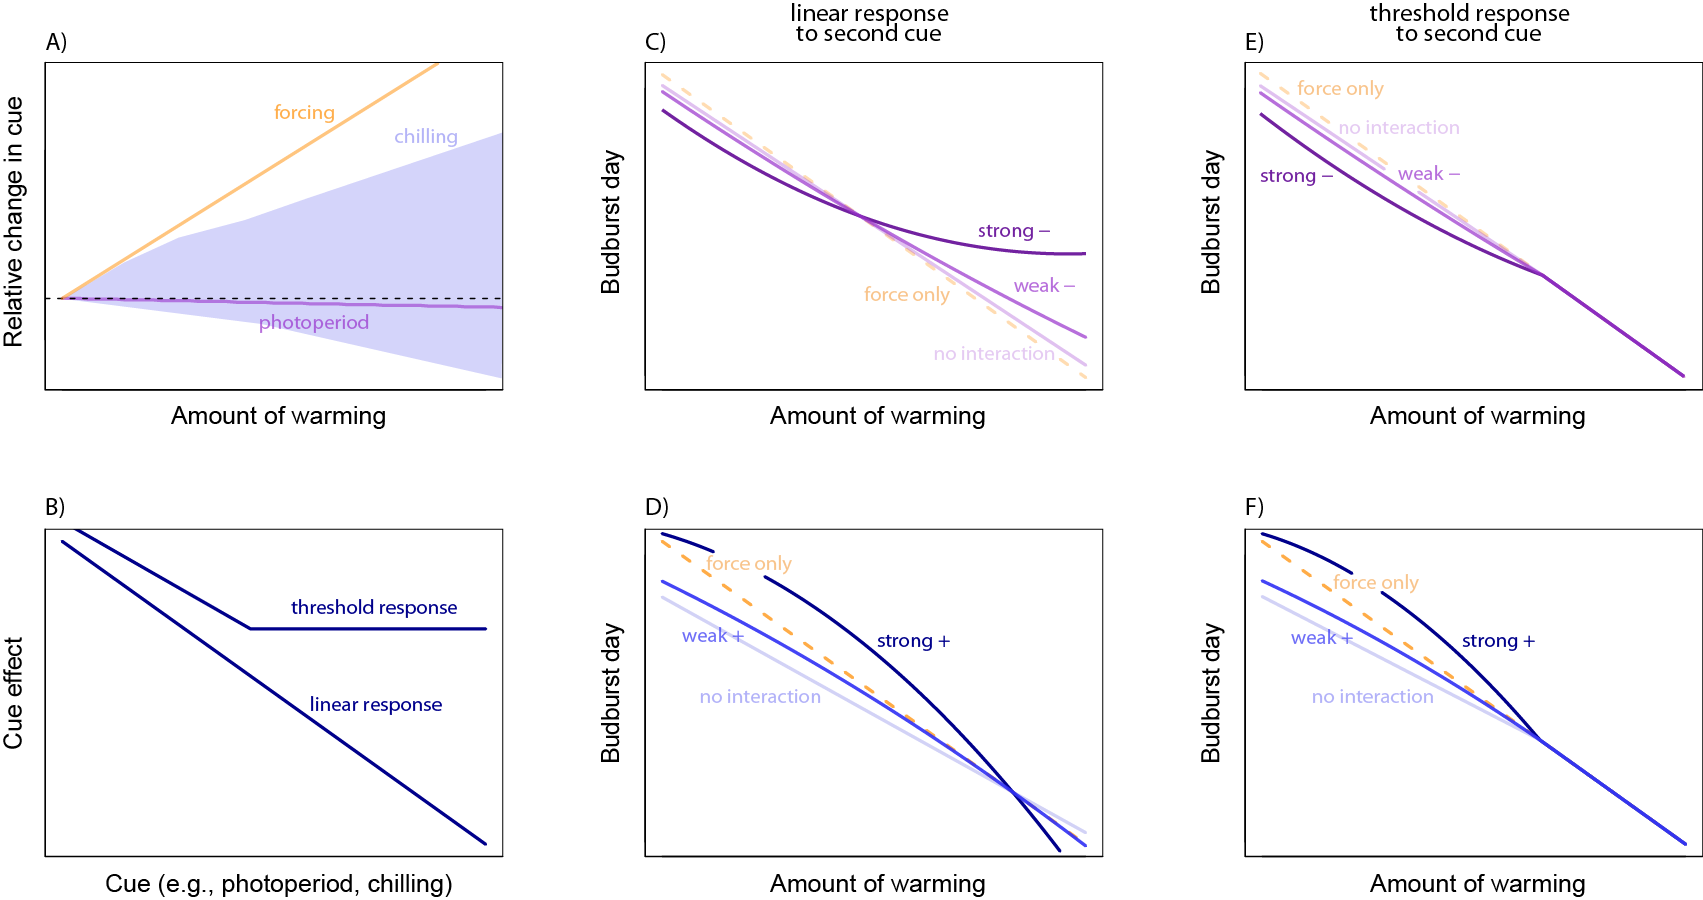
\includegraphics[width=1\textwidth]{..//..//analyses/limitingcues/figures/intxnsims2021photoaltwithchill_6panels_polyg_imc.png}
\caption{Interactions can produce nonlinearities, even in simple linear models if there are correlated shifts in cues. Much research focuses on how warming increases forcing (A), but it may also alter other cues, including photoperiod experienced near the time of the event, which is expected to shorten, and chilling, which may either increase or decrease (B). Shifts in forcing alongside shifts in a second cue (A) may produce non-linearities due to the interaction between cues (C-F showing the effect of: forcing-only in yellow, both cues without an interaction in lighter purple/blue, and both cues with an interaction in darker purple/blue); the overall change in budburst day predicted with warming depends on the sign ($+/-$), strength (weak/strong), and shape of the second cue (showing two simple examples: linear in C-D and threshold E-F).}
  \label{fig:intxncues}
\end{figure}
% Here we show examples considering a forcing x photoperiod interaction (top) and forcing x chilling (bottom), with both a linear effect of photoperiod or chilling (middle panels) or a threshold effect (left panels) versus an effect of forcing only (dashed gray line). These non-linearities come from the levels of both cues shifting at once: for the photoperiod example (top), as temperatures rise, forcing increases and the photoperiod experienced near the time of the event shortens (a similar response would be seen for lowering chilling), while for the chilling example (bottom), as temperatures rise forcing and chilling increases.}

\clearpage
\begin{figure}
\centering
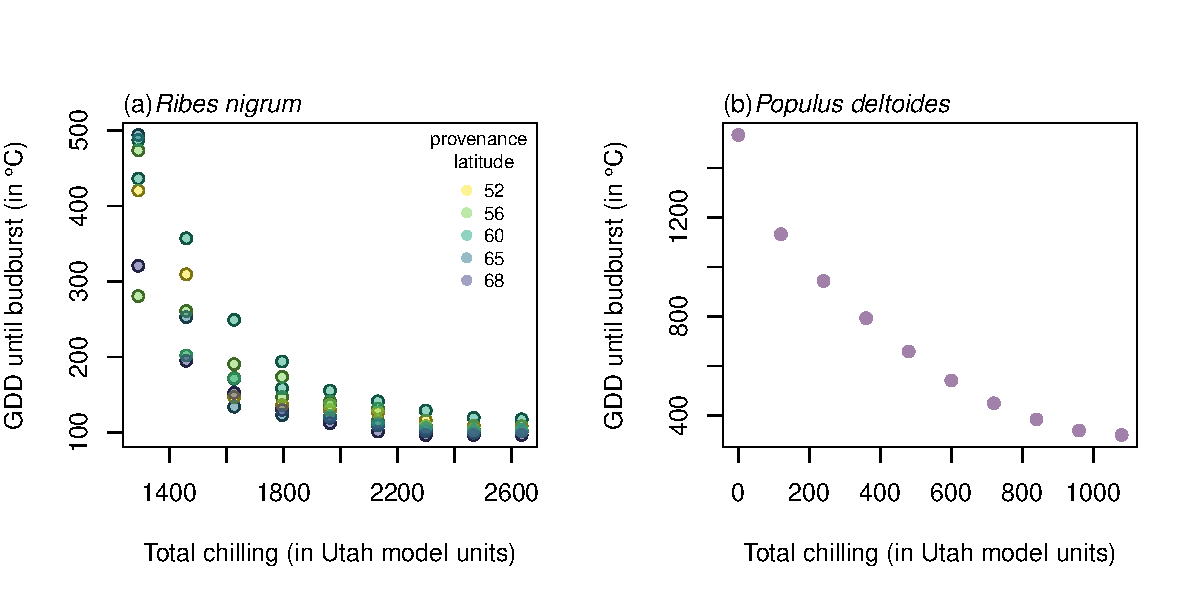
\includegraphics[width=1\textwidth]{..//..//analyses/limitingcues/figures/gddbyutahpretty.pdf}
\caption{A common example of how the level of one cue can modify the required level of another cue comes from experiments finding that the amount of chilling affects the amount of forcing needed for budburst. Here, we show this from experiments in black currant (\emph{Ribes nigrum}) from \citet{Sonsteby:2014aa} and eastern cottonwood (\emph{Populus deltoides}) from \citet{Thielges:1976aa}. Forcing is estimated as growing degree days (GDD, sum of temperatures $>0\degree$C) while chilling is estimated using the Utah Model \citep[see][]{richardson1974}.} % \citet{Cronje:2003aa} which studied apple (\emph{Malus sylvestris}), 
  \label{fig:gddbyutah} 
\end{figure}
% GDD_plottinglimcues.R

\clearpage
\begin{figure}[t!]
\centering
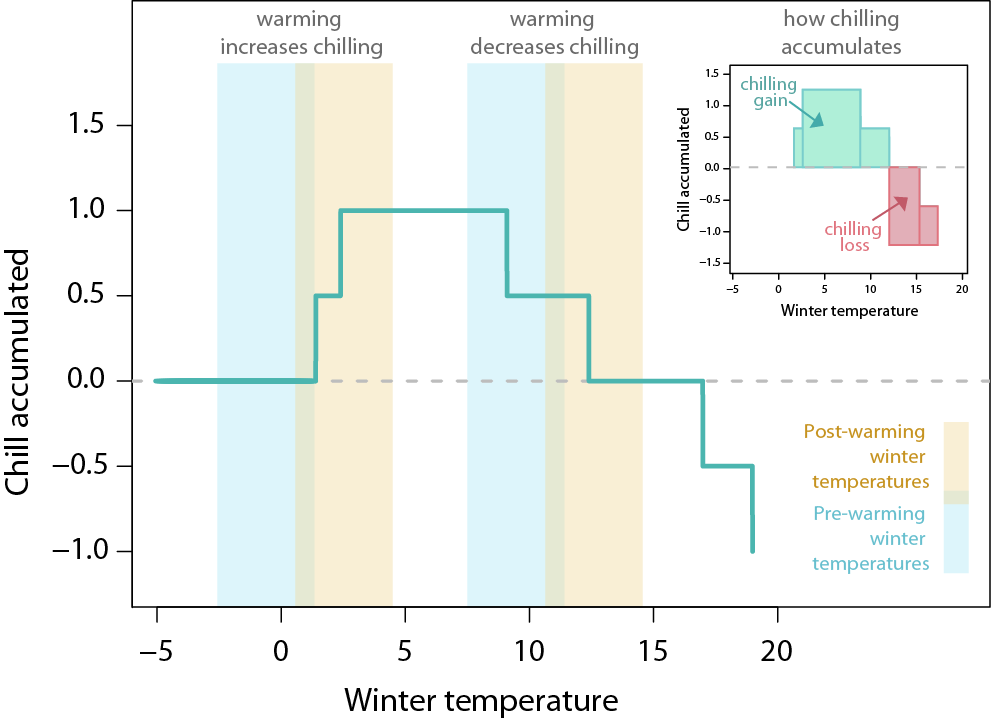
\includegraphics[width=0.6\textwidth]{figures/utahchill_limiting.png}
\caption{Current models of chilling suggest it may decrease or increase with winter warming. Here we show a common version of the Utah chilling model (top right inset and also turquoise line in main figure) with two conceptual scenarios of mean daily winter temperatures. When temperatures are generally below zero warming may increase accumulated chilling (left), while if pre-climate change temperatures are generally higher (near where chilling accumulates most per $\degree$C) then warming may decrease accumulated chilling (right).}
  \label{fig:chilling}
\end{figure}

\clearpage


\clearpage
\begin{figure}[t!]
\centering
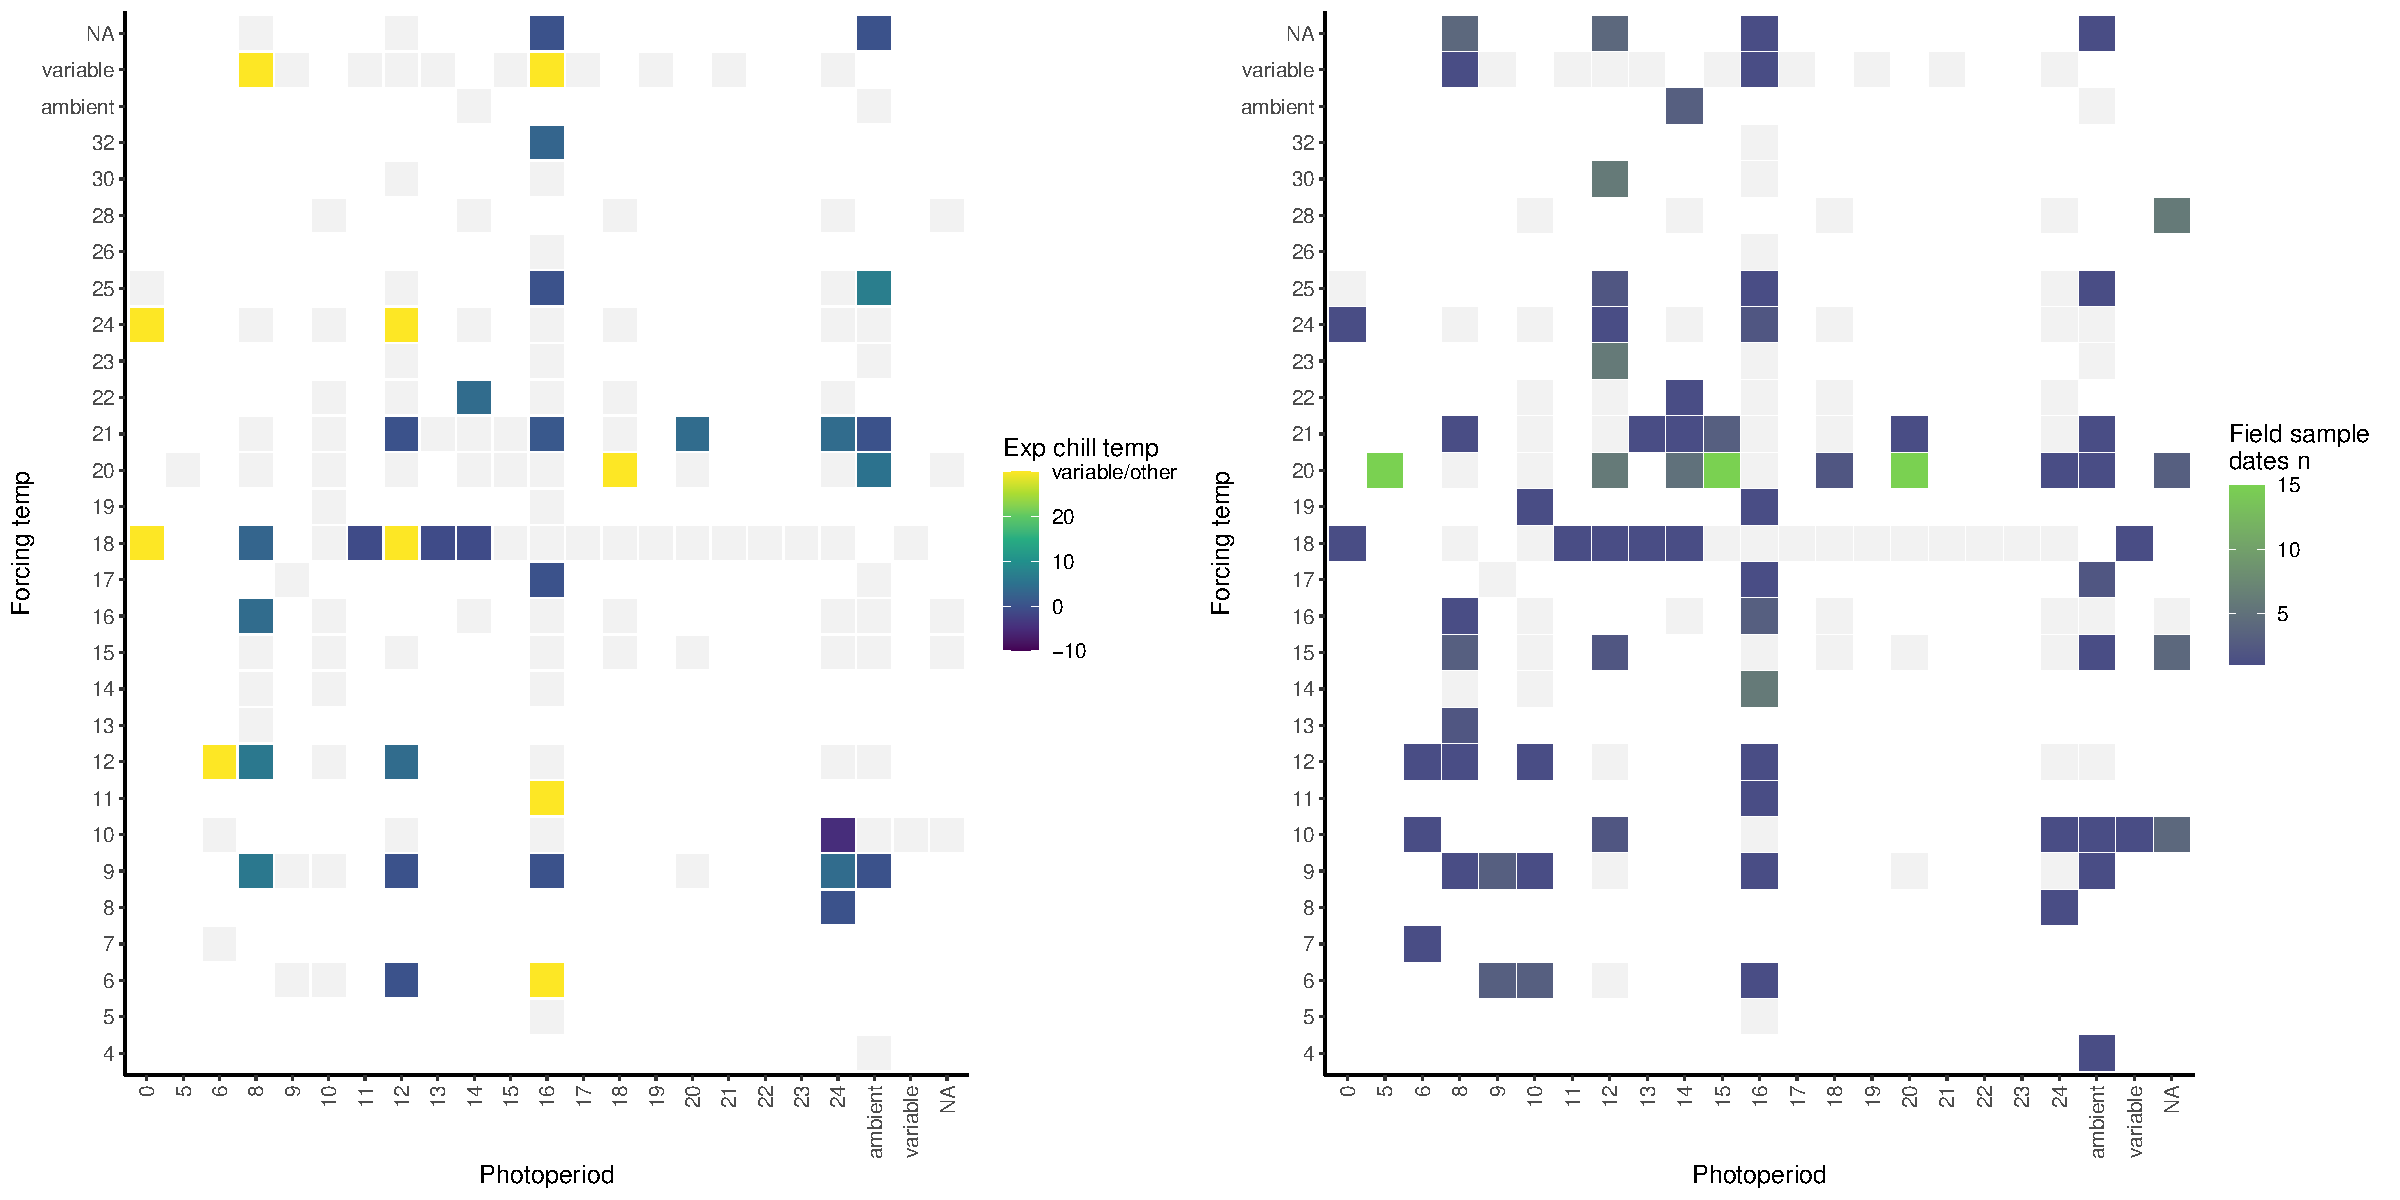
\includegraphics[width=1.1\textwidth]{..//..//analyses/limitingcues/figures/heatmapphotoxforcexchill2panel.pdf}
\caption{Studies have examined a range of cue-space (forcing temperature x photoperiod across two methods to manipulate chilling: a) experimentally or b) using multiple field sampling dates), but limited reporting of all cues makes using these data to estimate non-linearities challenging (see `Forecasting non-linear responses: Do we have the necessary data?'). Gray squares indicate a combination of forcing x photoperiod not present for that method of chilling design (includes studies that did not clearly define chilling treatments), while a value of `NA' indicates that we could not estimate a level of a particular cue because it was not clearly reported. Additionally, studies using `field chilling,' which take tissue (e.g., cuttings of adult dormant trees) from the field progressively across the fall and/or winter \citep[see][]{weinberger1950}, may assign changes in other cues to chilling. This is because such studies often equate tissue removed later as having received more chilling and thus often treat `time of cutting' as interchangeable with `chilling,'  though forcing and photoperiod conditions also change. Photoperiod treatments were generally only applied (or reported) during forcing conditions.}
  \label{fig:heatmaps} 
\end{figure}

\clearpage

\begin{figure}[t!]
\centering
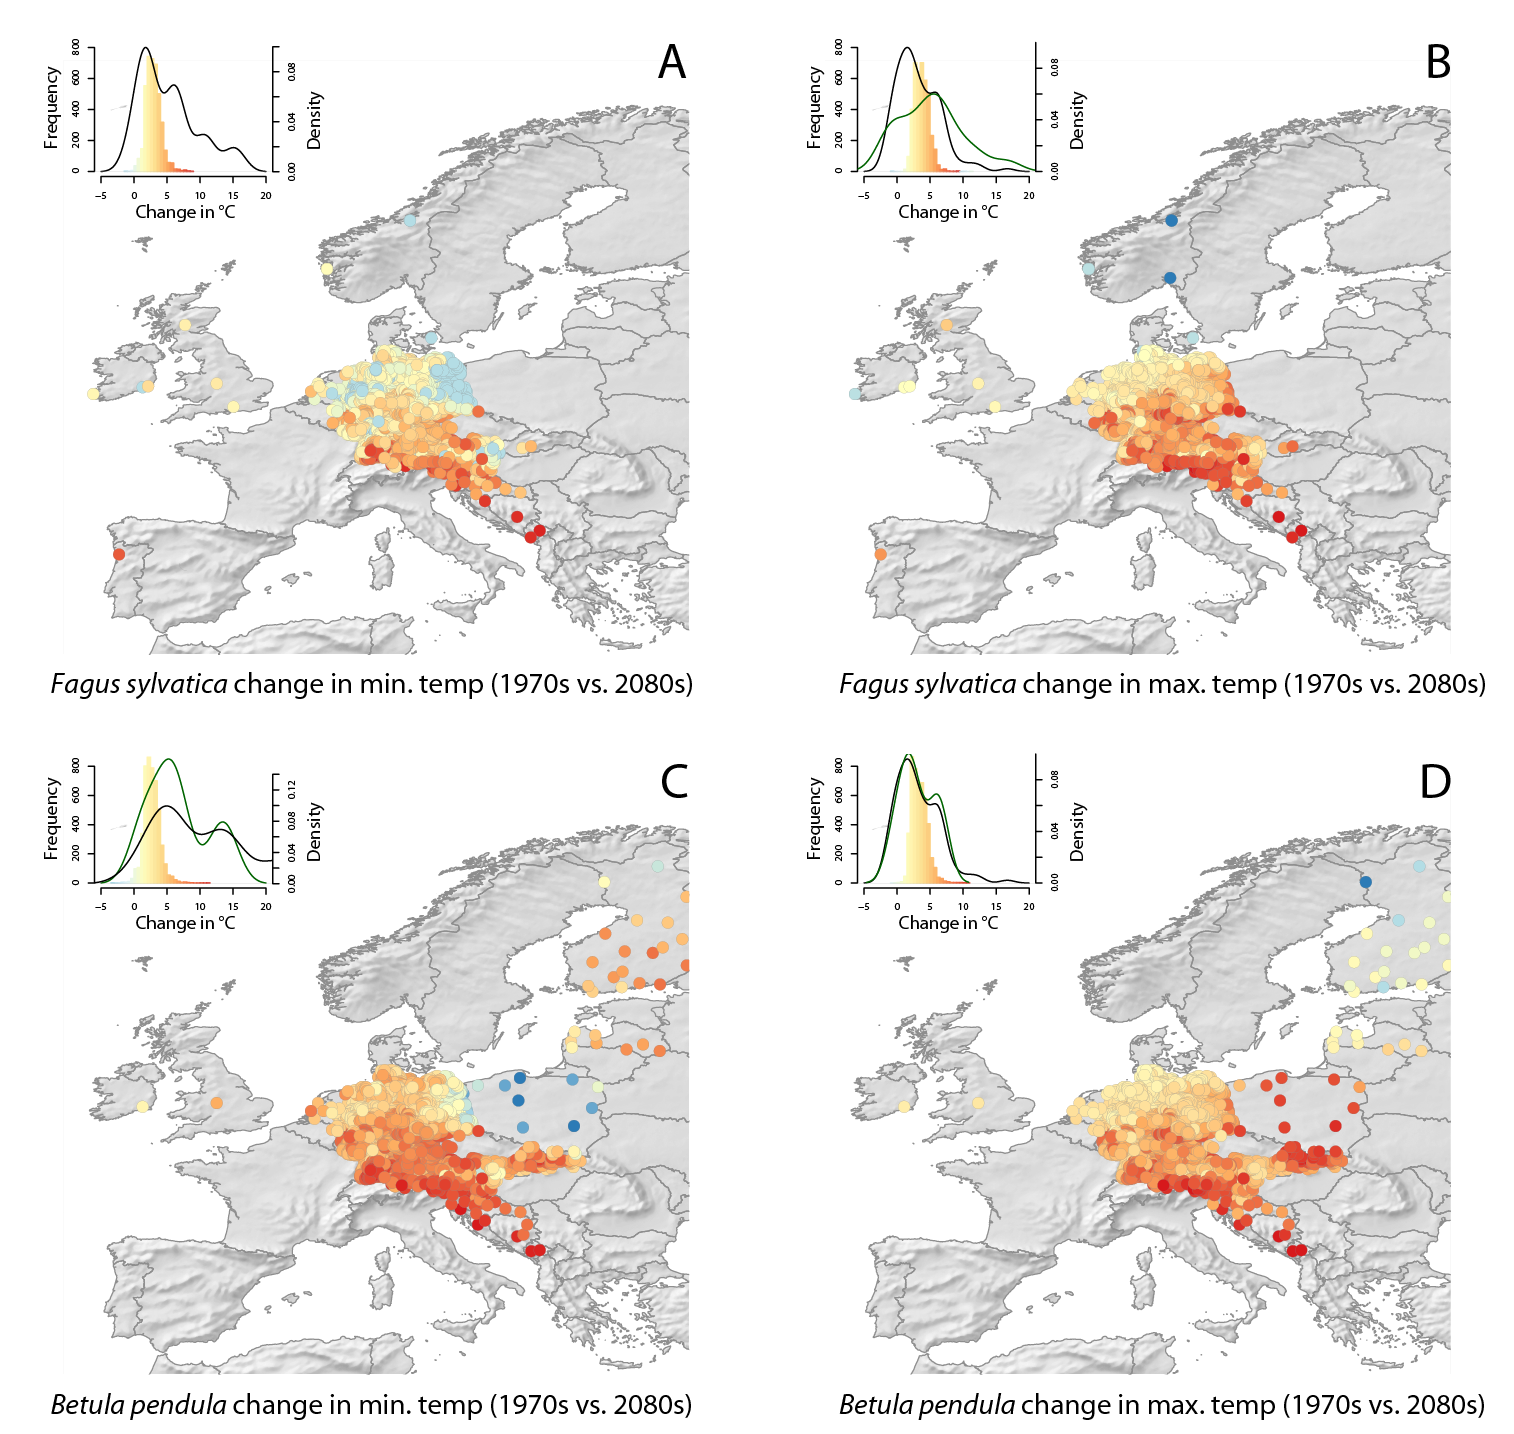
\includegraphics[width=1\textwidth]{figures/Fig7_noblues_densities.png}
\caption{Controlled environment studies' treatments are comparable to predicted temperature changes in the future for minima (A, C) and maxima (B, D). (C-D). Points represent a site with spring phenology data for each of two species, \emph{Fagus sylvatica} (A-B) and \emph{Betula pendula}, \citep[from the PEP725 database,][]{Templ2018} and show the predicted change (2080s average - 1970s average) in minimum (A,C) and maximum (B,D) temperatures 60 days before leafout. Inlay plots in the upper-left  corner of each plot show a histogram of these same predicted changes in temperature overlaid with densities of the chilling (A, C) and forcing (B, D) differences in treatments across studies (green lines show the treatments for that exact species, while black lines show across all species; for \emph{Fagus sylvatica} there are no chilling treatments of differing temperatures). For more details, see `Comparing experimental treatments to forecasted trends' in the Supporting Information.}
  \label{fig:pep} % studydesignplots.R
\end{figure}

\end{document}
